\section{Resultate}
\begin{figure}[hbt]
	\centering
		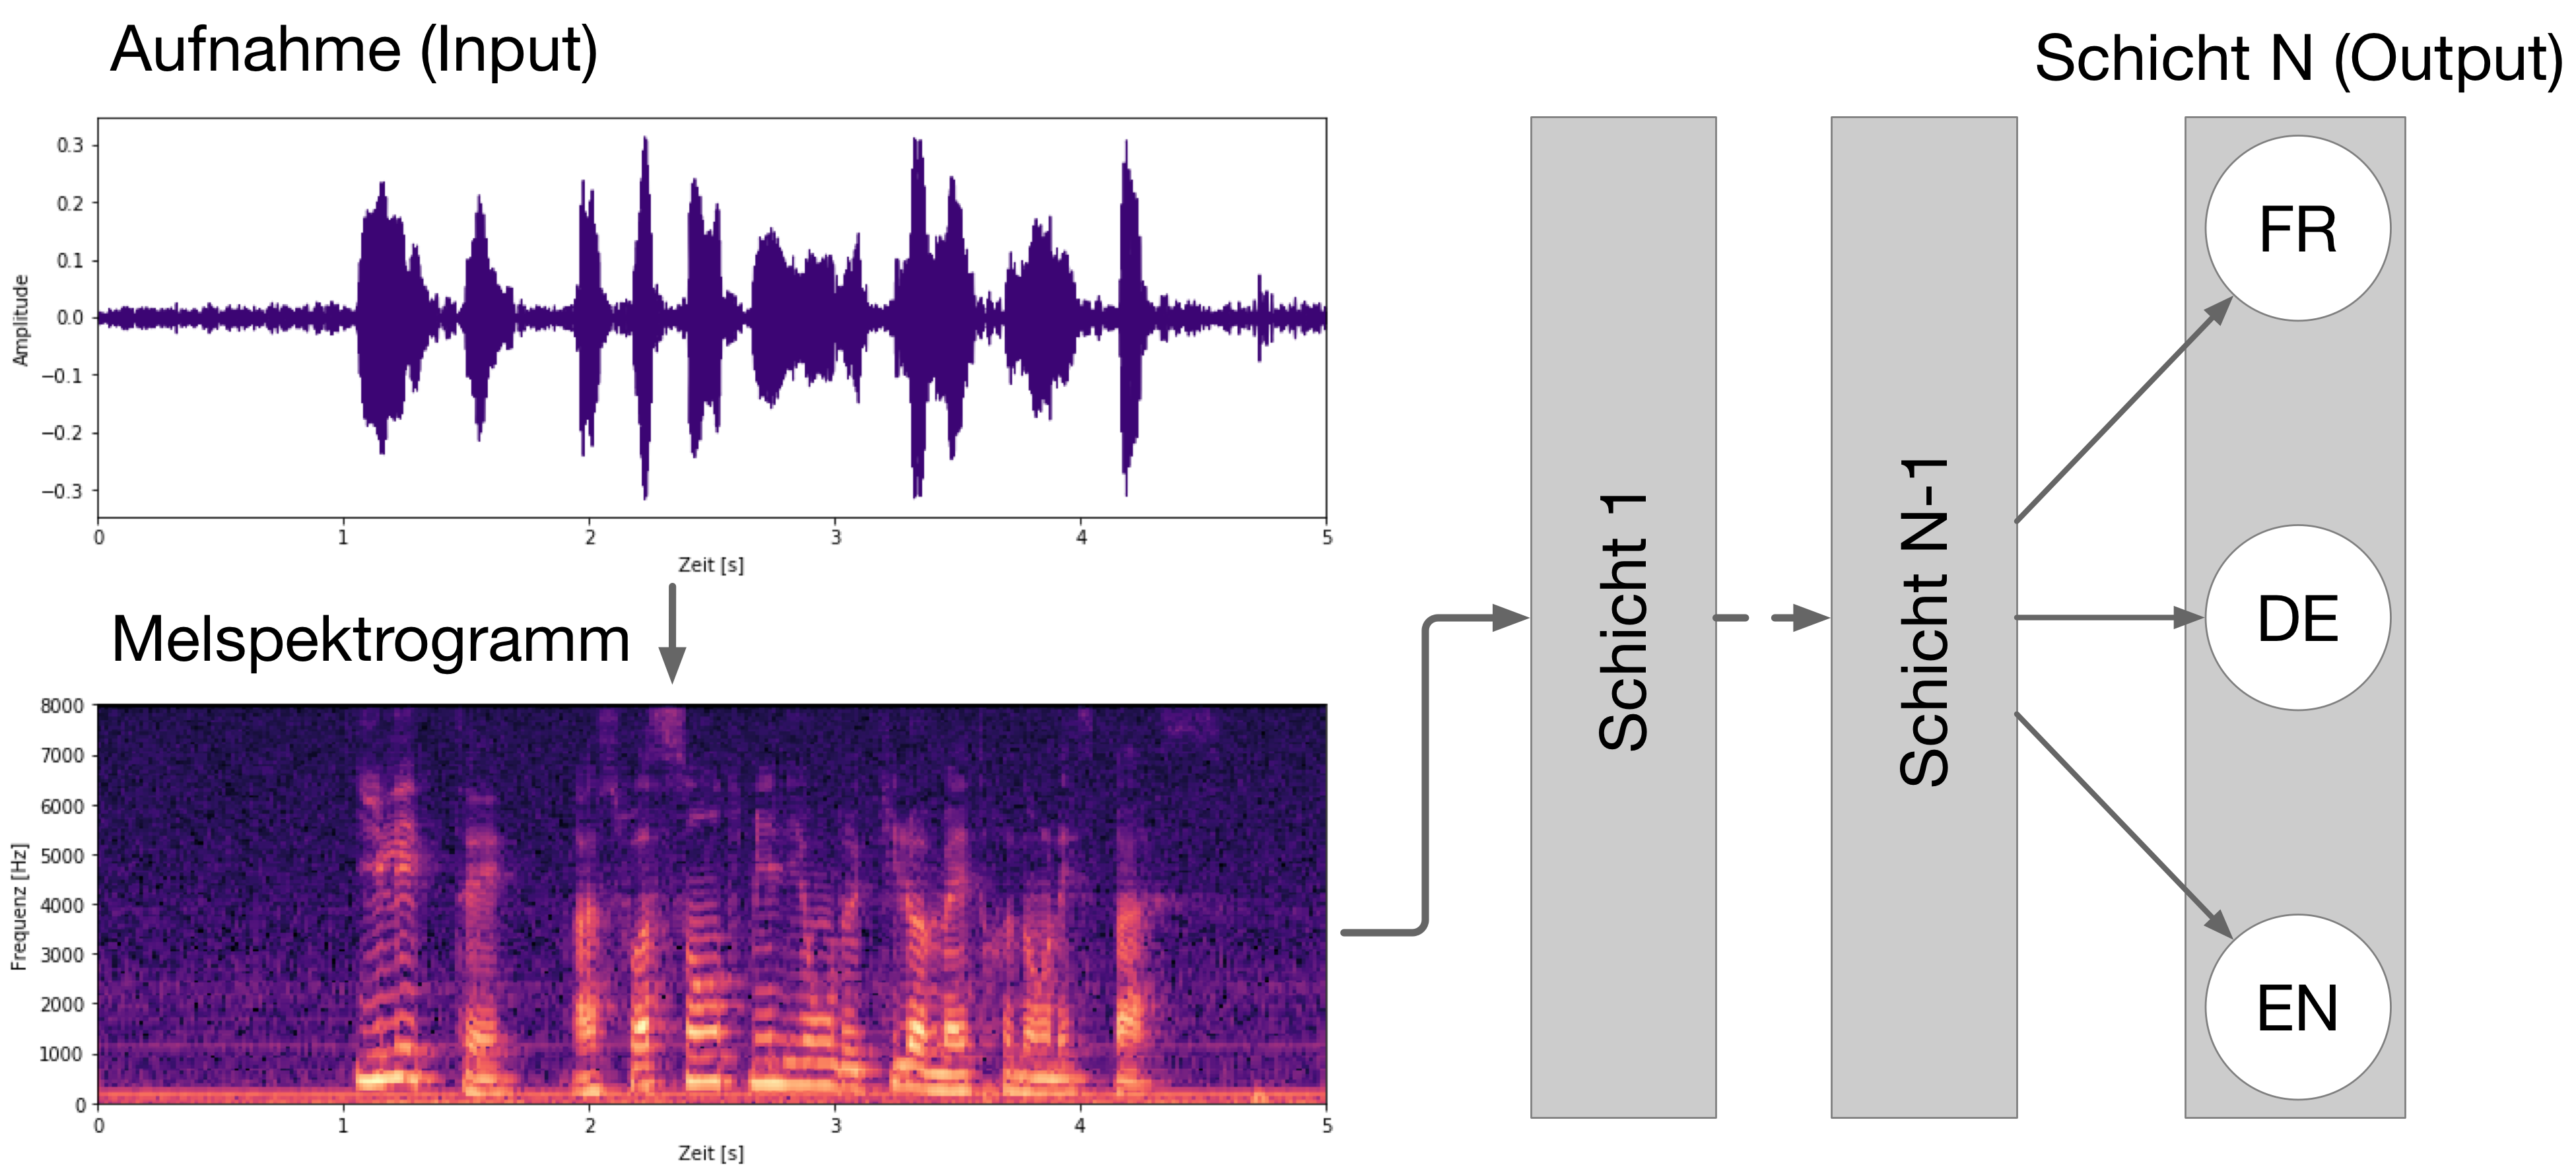
\includegraphics[width=0.8\textwidth]{assets/modelflow.png}
	\caption{Allgemeiner Aufbau}
	\label{img:workflow}
\end{figure}


\subsection{Modelle}

\subsubsection{CNN}
\begin{figure}[hbt]
	\centering
		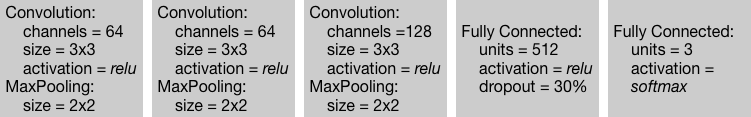
\includegraphics[width=0.8\textwidth]{assets/cnn.png}
	\caption{CNN Architektur}
	\label{img:cnn}
\end{figure}
basiert auf \parencite{iLID}

\subsubsection{InceptionV3-CNN}

\subsubsection{CRNN}
basiert auf \parencite{crnn}

\subsubsection{GAN}
basiert auf \parencite{gan}

\subsection{Auswertung}

\subsubsection{Auf Test-Datenset}

\begin{table}[h]
	\centering
	\begin{tabular}{llll}
		\hline
		Netz & Architektur     & Accuracy & Loss  \\ \hline
		CNN  & 3 Conv          & 90\%     & 0.02  \\
		CRNN & 4 Conv + LSTM   & 94\%     & 0.015 \\
		CNN  & 28 Conv + Dense & 87\%     & 0.03  \\ \hline
	\end{tabular}
	\caption{Top Accuracy}
	\label{table:test}
\end{table}

\subsubsection{Auf Beta-Datenset}